\documentclass[border=2pt]{standalone}
% Shared preamble of the standalone figures of Paper2_V28 (journal artwork rules: Helvetica
% lettering, 8-9 pt at final size, lines >= 0.4 pt, colorblind-safe RGB colors plus patterns).
\usepackage[T1]{fontenc}
\usepackage[scaled=0.95]{helvet}
\renewcommand{\familydefault}{\sfdefault}
\usepackage[helvet]{sfmath}
\usepackage{textcomp}
\usepackage{tikz}
\usepackage{pgfplots}
\pgfplotsset{compat=1.17}
\usetikzlibrary{arrows.meta,calc,positioning,patterns}
\definecolor{okblue}{HTML}{0072B2}
\definecolor{okverm}{HTML}{D55E00}
\definecolor{okgray}{HTML}{9A9A9A}
\definecolor{oklight}{HTML}{D9D9D9}
\definecolor{okdark}{HTML}{4D4D4D}

\begin{document}
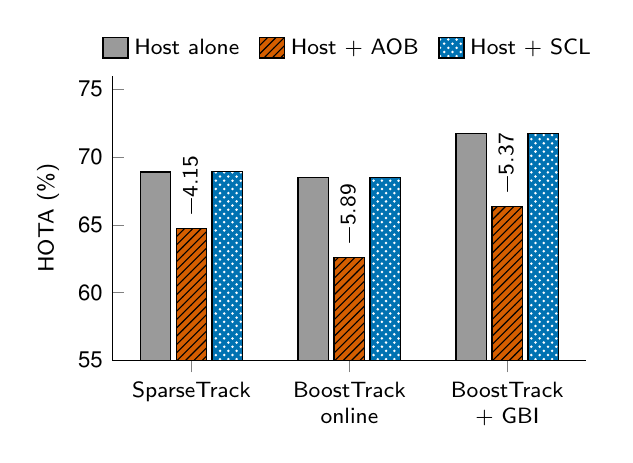
\begin{tikzpicture}
\begin{axis}[
  ybar, /pgf/bar width=11pt, width=7.6cm, height=5.2cm,
  ymin=55, ymax=76, xmin=0.5, xmax=3.5,
  xtick={1,2,3},
  xticklabels={SparseTrack, {BoostTrack\\online}, {BoostTrack\\+ GBI}},
  xticklabel style={align=center},
  ylabel={HOTA (\%)},
  axis x line*=bottom, axis y line*=left, axis line style={line width=0.6pt},
  tick label style={font=\footnotesize}, label style={font=\footnotesize},
  legend style={at={(0.5,1.02)}, anchor=south, legend columns=3, font=\footnotesize, draw=none,
    /tikz/every even column/.append style={column sep=5pt}},
  legend image code/.code={\draw[#1] (0cm,-0.12cm) rectangle (0.32cm,0.14cm);},
  legend cell align=left,
]
\addplot[fill=okgray, draw=black, line width=0.5pt] coordinates {(1,68.88) (2,68.49) (3,71.72)};
\addplot[fill=okverm, draw=black, line width=0.5pt, postaction={pattern=north east lines, pattern color=black}] coordinates {(1,64.72) (2,62.61) (3,66.35)};
\addplot[fill=okblue, draw=black, line width=0.5pt, postaction={pattern=crosshatch dots, pattern color=white}] coordinates {(1,68.93) (2,68.49) (3,71.72)};
\legend{Host alone, Host + AOB, Host + SCL}
\node[rotate=90, anchor=west, font=\footnotesize] at (axis cs:1,64.95) {\textminus 4.15};
\node[rotate=90, anchor=west, font=\footnotesize] at (axis cs:2,62.85) {\textminus 5.89};
\node[rotate=90, anchor=west, font=\footnotesize] at (axis cs:3,66.6) {\textminus 5.37};
\end{axis}
\end{tikzpicture}
\end{document}
